\section{Crosscutting Concept}

In this chapter we will present the technical solutions that we will use to develop this project.
For each quality attribute we will present the chosen tactitcs.

\subsection{Solutions for Usability}

\subsection{Solutions for Interoperability}

The communication with the 3rd party components should during the whole lifetime of the App reliable. Since we are dealing with
two different services, \gls{mobile payment gateway} and \gls{federated login}, we will describe the integration processes 
according to each specification.

From the third party applications we expect the following interaction:

\begin{figure}[H]
    \centering
    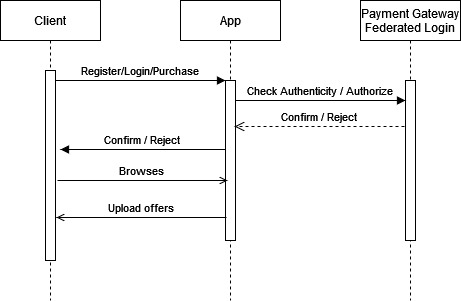
\includegraphics[width=0.7\textwidth]{assets/sequence_login_payment.jpg}
    \caption{Sequence of actions with 3rd party applications}
    \label{fig:sequence_login_payment}
\end{figure}

\subsubsection{Payment Gateway}

The usage of \gls{mobile payment gateway} offers three possibilities \cite{refonline:ZOPG}:

\begin{itemize}
    \item Redirection to payment processor's page
    \item Payment data and processing inside the application
    \item Payment data entered in the app, but processed with an \acrshort{api}
\end{itemize}

The third option stays in direct contact with our top quality attribute, usability. Since we want to offer a easy shopping
experience, the payment process should also be harmonic with other features.

\begin{table}[H]
    \setstretch{1.0}
    \begin{tabularx}{\textwidth}{|c|c|X|}
        \toprule
        \multicolumn{1}{c}{Tactict} & \multicolumn{1}{c}{Pattern} & \multicolumn{1}{c}{Motivation} \\
        \midrule
        \textbf{Limit Dependencies} & Wrapper & The \gls{api} will be the intermediary for the payment process. For the 
        \glsplural{client} all visible steps will occur in the app, without being sent to another page. On the background
        the \gls{api} will receive the input and send it to the payment gateway. The verification takes place in gateway, 
        which then communicate with the financial institute of the client and send the payment to the \gls{provider} 
        \cite{refonline:ZOPG}.  \\
        \bottomrule
    \end{tabularx}
\end{table}




\subsection{Solutions for Performance}